\section{Motivación}

Los sistemas de transporte conforman la columna vertebral de nuestras ciudades, contribuyendo directamente al desarrollo de la sociedad urbana. Un sistema de transporte bien diseñado y eficiente permite el desplazamiento rápido y cómodo de personas y bienes; en cambio, uno ineficiente genera grandes problemas, alargando los tiempos de viaje y aumentando la contaminación atmosférica.

Los Sistemas de Transporte Inteligente surgen como una respuesta a la necesidad de optimización, modernización y mejoramiento de los sistemas de transporte ya existentes. La Unión Europea define a los ITS como aplicaciones que pretenden proveer servicios innovadores relacionados con distintos modos de transporte y de administración de tráfico, que además otorgan información a los usuarios y les permiten utilizar el sistema de transporte de manera más segura, coordinada e inteligente \cite{eudirective}. Esta amplia definición abarca una gran cantidad de aplicaciones: desde sistemas de alerta temprana a sistemas de entretención en ruta, pasando incluso por aplicaciones tan avanzadas como sistemas de coordinación y control de vehículos autónomos -- la figura \ref{fig:itsetsi} ilustra algunas de éstas. 

\begin{figure}[tpb]
    \centering
    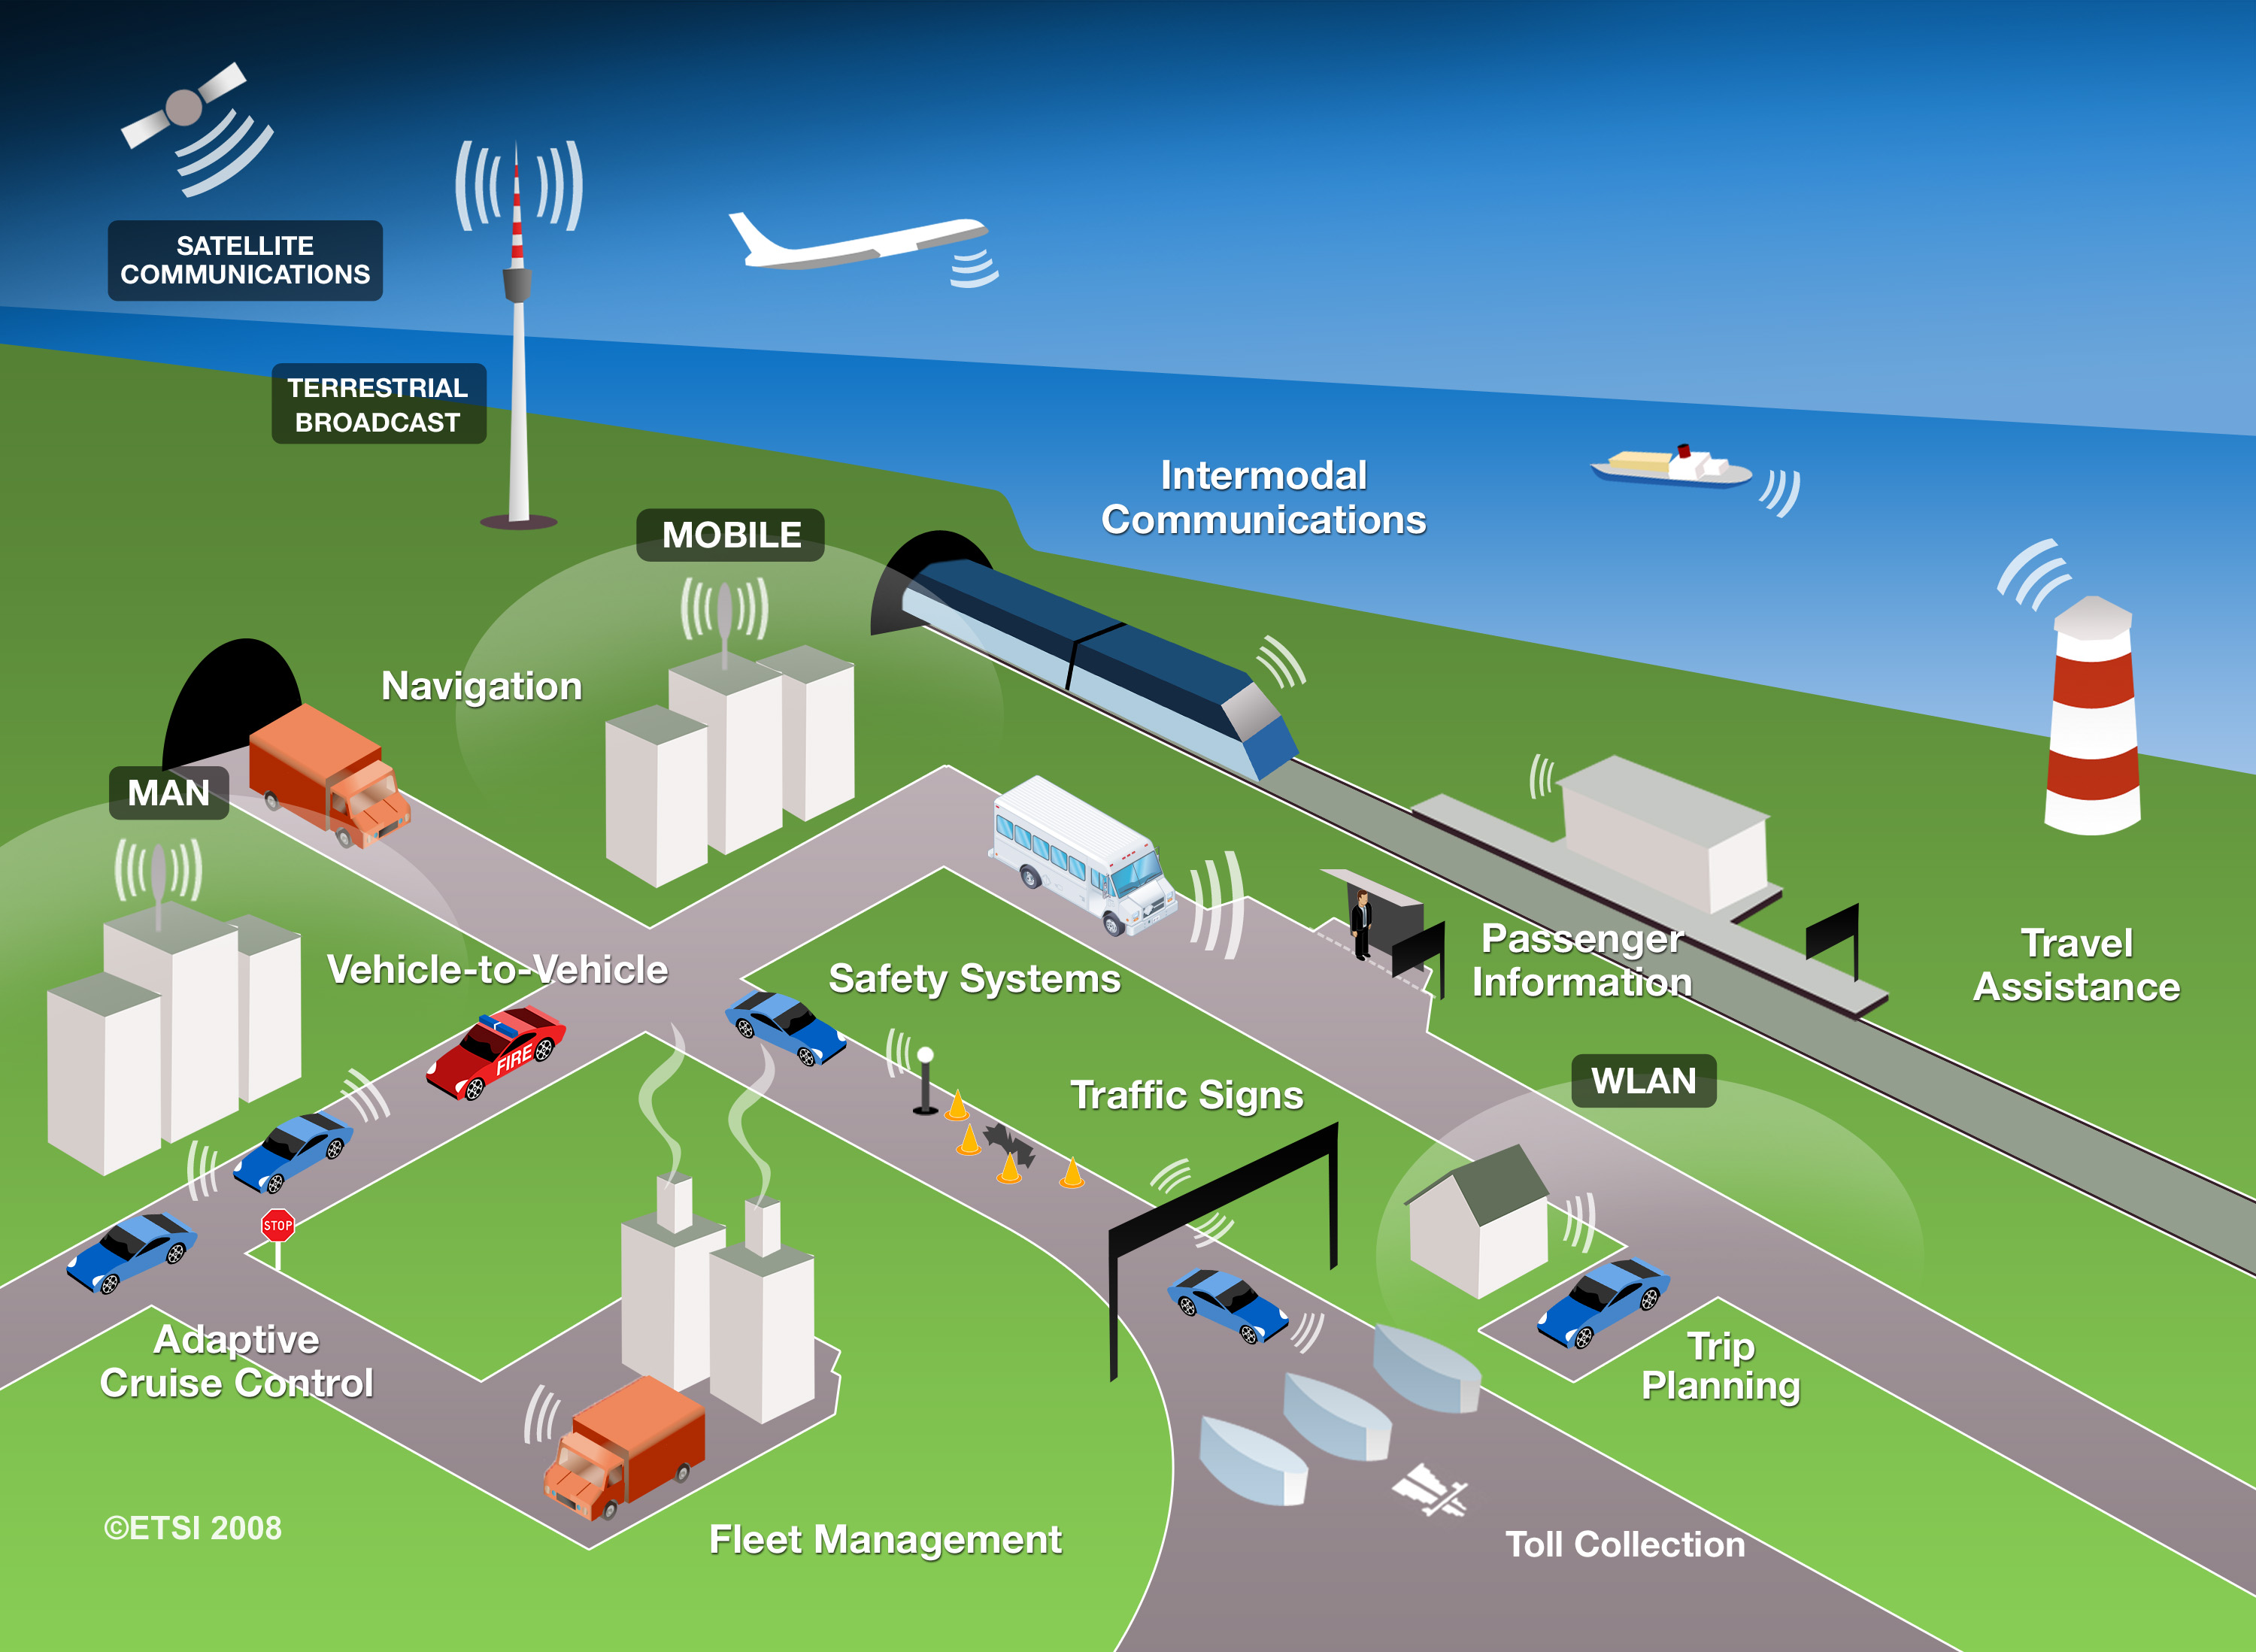
\includegraphics[width=0.9\linewidth]{figuras/ITS.png}
    \caption{Aplicaciones en un Sistema Inteligente de Transporte (fuente: ETSI \autocite{etsi}).}
    \label{fig:itsetsi}
\end{figure}

El factor común entre todas estas aplicaciones es la necesidad de extraer información en tiempo real desde el entorno, la cual debe procesarse y en muchos casos generar una respuesta a transmitir al usuario. Para este fin, se ha propuesto la implementación de tecnologías que posibiliten esta comunicación, principalmente utilizando redes inalámbricas, tanto de área local (los estándares incluídos en la familia WLAN, IEEE 802.11), como de área personal (WPAN, IEEE 802.15) \cite{80211dailey,80215vanet,80211wave}. Sin embargo, estas tecnologías fueron diseñadas originalmente para su uso en redes estáticas o con patrones de movimiento muy limitados, y es necesaria la evaluación de su desempeño en entornos altamente dinámicos como lo son los sistemas de transporte vehicular. Parámetros críticos para el funcionamiento óptimo de la red, como la potencia de transmisión, las condiciones del canal de transmisión y la distancia óptima entre nodos, deben establecerse teniendo en cuenta las particularidades que presentan los sistemas de transporte -- por ejemplo, la alta congestión de nodos en intersecciones con semáforos.

Existe entonces hoy en día la necesidad de modelar de manera realista y precisa el comportamiento de estas tecnologías en contextos de comunicaciones inalámbricas en redes vehiculares. Por otro lado, existe también la necesidad de modelar el impacto de la comunicación inalámbrica en un sistema de transporte, y cómo esta puede contribuir a optimizar la operación del mismo \cite{bidirectionalsimul}. Un ejemplo de esto son los Sistemas Avanzados de Información al Viajero (\textit{ATIS}, por sus siglas en inglés; \textit{Advanced Traveller Information System}) los cuales proveen información en tiempo real sobre las condiciones del tránsito a conductores, permitiéndoles elegir la ruta más óptima para alcanzar su destino. Este \textit{feedback} inmediato sin duda tiene efectos importantes en el flujo vehicular de un sistema de transportes, los cuales deben ser tomados en consideración al momento de modelar y simular el funcionamiento del mismo.